% 1984 年全国卷（理科）第 20 题：半径为 1 的圆与直线 l 相切于 A，动点 P 沿 l 右移，直线 PC 交直线 AO 于 M（按源卷布局）。
% 取坐标 A=(0,0)、圆心 O=(0,1)；图示时刻取弧 AC 对应圆心角 75°，C 落在圆上右下方，M 在 O 上方。
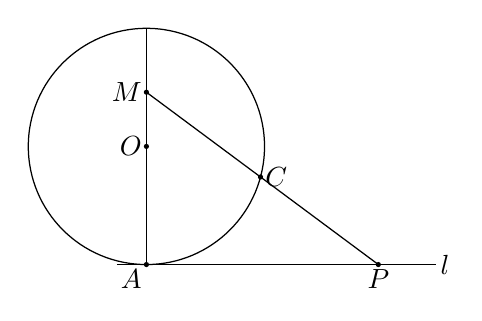
\begin{tikzpicture}[scale=1.5, line width=0.45pt,
  every node/.style={inner sep=1.5pt}]
  \coordinate (A) at (0,0);
  \coordinate (O) at (0,1);
  \coordinate (T) at (0,2);          % 直径上端点
  \coordinate (P) at (1.9635,0);     % 动点 P（在 l 上，A 之右）
  \coordinate (C) at (0.9659,0.7412); % 圆上点 C（弧 AC 长 = 2/3·AP）
  \coordinate (M) at (0,1.4589);     % 直线 PC 与直线 AO 的交点
  \draw (O) circle (1);
  \draw (-0.25,0) -- (2.45,0);       % 切线 l
  \draw (A) -- (T);                  % 直线 AO（过 A 的直径）
  \draw (P) -- (M);                  % 直线 PC（M、C、P 共线）
  \fill (A) circle (0.022);
  \fill (O) circle (0.022);
  \fill (P) circle (0.022);
  \fill (C) circle (0.022);
  \fill (M) circle (0.022);
  \node[left] at (M) {$M$};
  \node[left] at (O) {$O$};
  \node[below left] at (A) {$A$};
  \node[below] at (P) {$P$};
  \node[right] at (C) {$C$};
  \node[right] at (2.45,0) {$l$};
\end{tikzpicture}
